\begin{frame}{Los ingresos tributarios aumentaron a 14,7\% del PIB en 2025}
\centering
\resizebox{0.90\textwidth}{!}{
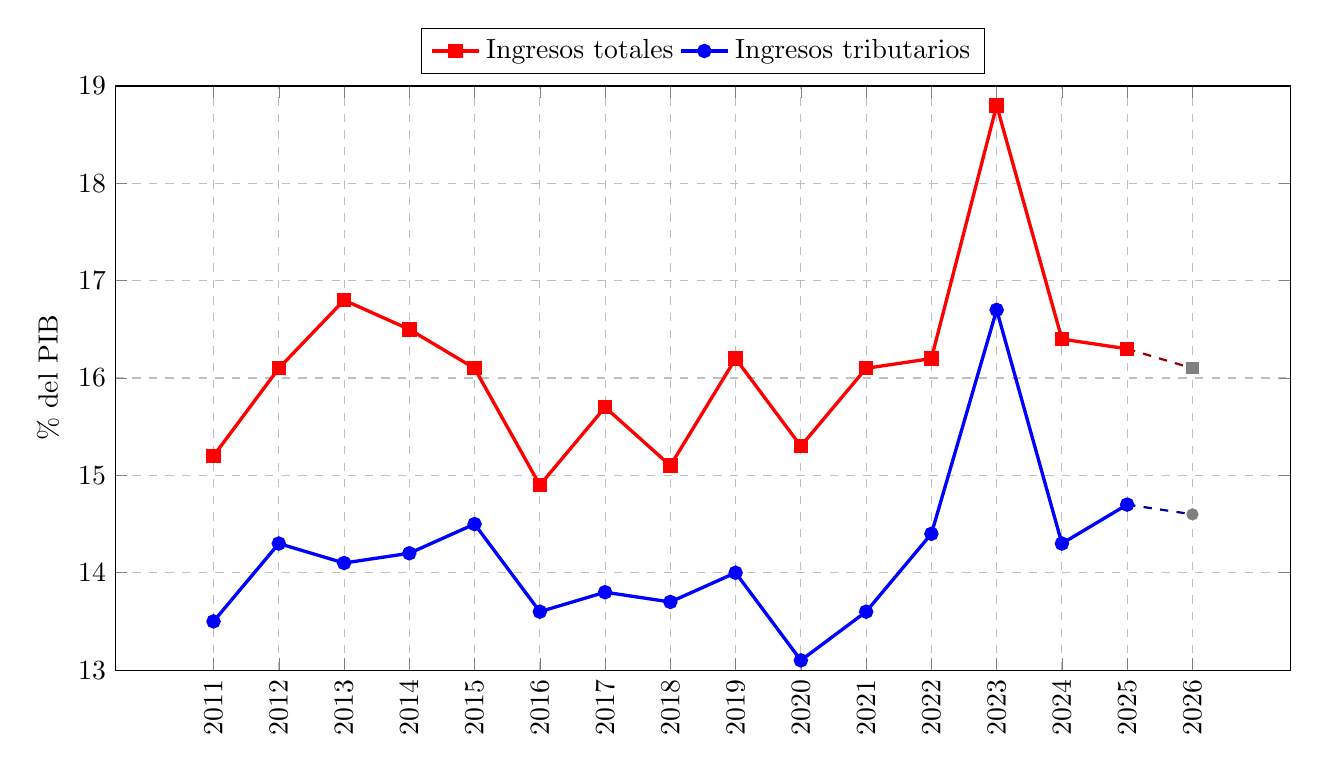
\begin{tikzpicture}
\begin{axis}[
    width=16.5cm,
    height=9cm,
    ylabel={\% del PIB},
    xtick={7,8,...,22},
    xticklabels={2011,2012,2013,2014,2015,2016,2017,2018,2019,2020,2021,2022,2023,2024,2025,2026},
    x tick label style={rotate=90,anchor=east},
    ymin=13,
    ymax=19,
    grid=both,
    grid style=dashed,
    legend style={at={(0.5,1.02)},anchor=south,legend columns=-1}
]
\addplot[color=red,mark=square*,very thick] coordinates {
    (7,15.2) (8,16.1) (9,16.8) (10,16.5) (11,16.1) (12,14.9)
    (13,15.7) (14,15.1) (15,16.2) (16,15.3) (17,16.1) (18,16.2)
    (19,18.8) (20,16.4) (21,16.3)
};
\addlegendentry{Ingresos totales}
\addplot[color=blue,mark=*,very thick] coordinates {
    (7,13.5) (8,14.3) (9,14.1) (10,14.2) (11,14.5) (12,13.6)
    (13,13.8) (14,13.7) (15,14.0) (16,13.1) (17,13.6) (18,14.4)
    (19,16.7) (20,14.3) (21,14.7)
};
\addlegendentry{Ingresos tributarios}
\addplot[color=red!60!black,dashed,thick] coordinates {(21,16.3) (22,16.1)};
\addplot[color=blue!60!black,dashed,thick] coordinates {(21,14.7) (22,14.6)};
\addplot[color=gray,mark=square*,only marks] coordinates {(22,16.1)};
\addplot[color=gray,mark=*,only marks] coordinates {(22,14.6)};
\end{axis}
\end{tikzpicture}}
\scriptsize Línea sólida: resultados observados hasta 2025. Línea discontinua: proyección 2026.
\note{[Sources] MFMP 2026, capítulo 1, tablas 1.3 y 1.4. Serie histórica previa: MHCP, como en la versión fuente.}
\end{frame}